% !TEX root = template.tex

% some macros
\newcommand*{\x}{\boldsymbol{x}}
\newcommand*{\y}{\boldsymbol{y}}
\newcommand*{\z}{\boldsymbol{z}}
\newcommand*{\xm}{\bar{\x}}

\newpage

\section{Processing Pipeline}
\label{sec:processing-pipeline}

\begin{figure*}[h]
	\centering
	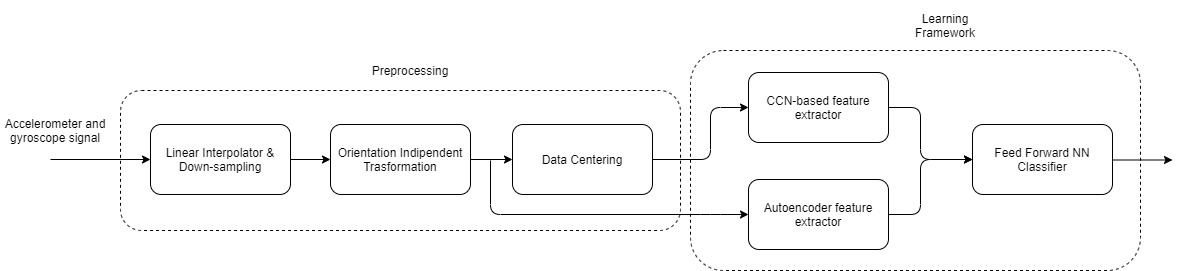
\includegraphics[width=1\textwidth]{images/processing_pipeline.jpg}
	\caption{Processing pipeline}
\end{figure*}

The task of HAR in real use case scenarios is a difficult task, and many aspects need to be considered when these applications are brought in a mobile environment. As reported in \cite{blunck2013heterogeneity} the three major types of heterogeneties which yield impairments in HAR are:
\begin{itemize}
	\item \textbf{Sensor Biases (SB)}: To keep the overall cost of a smartphone low, low costs accelerometer and gyroscope sensor are used, yielding a poor-calibrated, inaccurate and range/granularity limited acquired signals. So, among this type of sensors we could observe differences in precision, resolution, range and also biases. Usually an initial sensors calibration is made by smartphones manufactures, but due to rotation or misalignment of sensor to the circuit board errors can be introduced. Furthermore, if a device experiences shock, e.g falling on the ground, the sensor can be misaligned causing unwanted biases.
	\item \textbf{Sampling Rate Heterogeneity (SRH)}: Often popular smartphones vary in terms of default and supported sampling frequencies for accelerometer and gyroscope sensor. In the dataset TODO riportare link used for this experiment for example we are dealing with smartphone where the sampling frequency varies from 50Hz to 200Hz. See Fig. TODO so the actual number of devices used in this dataset, with their corresponding sampling frequencies.
	\item \textbf{Sampling Rate Instability (SRI)}: This phenomenon is specific to a single device and regards the regularity of time span between successive measurements. Different factors could accentuate this problem, including heavy multitasking or high I/O load in the mobile device. Multitasking effect in particular is a major problem: smartphone usually prioritizes among various running tasks and doing so could extremely affects the sensor sampling of a HAR application running on the device. In our collected dataset with a 100 Hz sampling rate (which means a time-span between consecutive samples of $10ms$), for example we observe time-span ranging mainly between $3ms$ and $15ms$ with an average of $7ms$. Although in our collected dataset the smartphone was set in \textit{airplane mode} to reduce at minimum this effect. The Fig. \ref{time-span} shows the amount of different time-span present in our dataset.
\end{itemize}

\begin{figure}[h]
	\centering
	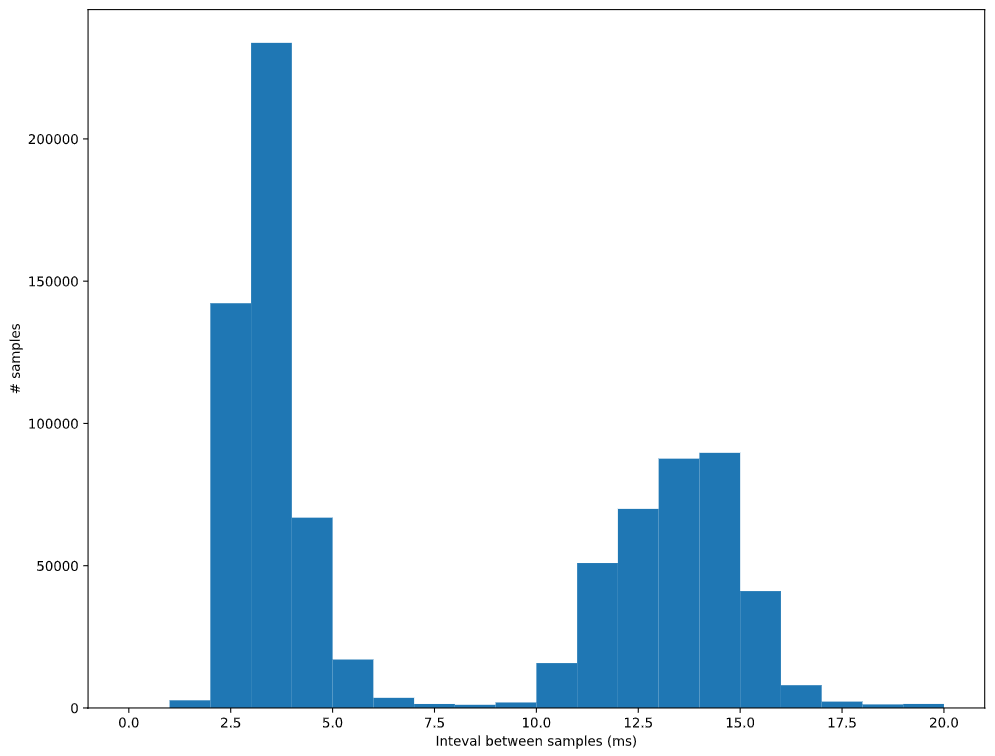
\includegraphics[width=0.4\textwidth]{images/interval_samples.png}
	\caption{Histogram of different time span between samples included in our collected dataset}
	\label{time-span}
\end{figure}

Furthermore, if we considered a real use case scenarios of a HAR mobile application we must also consider that smartphones can be positioned and oriented in different ways in human body. For example a smartphone could lay in trouser pockets (back and front) or maybe inside a pouch or a bag with different orientations. These different initial model settings have huge effects in prediction accuracy of an HAR predictor, especially if the model has been trained on a dataset that consist of activity measurement coming from only one fixed position and orientation of the smartphone, as is usually the case dealing with dataset collected in a controlled environment that could be found on Internet.\footnote{TODO: magari mettaimo ``that ara available in literature''?}

To tackle all these problems we decided to adopt in our pre-processing pipeline as show in Fig. TODO, 3 main blocks.

The first block called Linear Interpolator is in charge of mitigate the problems regarding the SRH and SRI as discussed previously. It main purpose is to down-sample the input data to a fixed sampling rate, in our case 50 samples/second.

The second block called Orientation Independent Transformation is used to represent data coming from different orientation of the smartphone in a rotation independent space. In this way all the signals are projected in a new space whose orientation is independent of that of the smartphone and aligned with gravity and the direction of motion. In this way an user can place his smartphone in whatever position he or she wants, mitigating the problem of different position and rotations of smartphone, as we will see in the Experiment section TODO reference.

Our last block consists of a data centering operation, applied for centering signals among y-axis that are presented only for the Covolutional Layer and not for the Autoencoder block. The reason of this choice would be clear in the section TODO. As reported in \cite{ignatov2018real}, time series centering standardize the input data, making the task for the CNN easier. Data normalization instead must be avoided because does not help in this situation since it significantly distorts time series shape, removing magnitude information which is critical for activities differentiation.

After the preprocessing pipeline we adopt a novel Learning framework. It is composed of CNN augmented with features coming from an autoencoder. As discussed in \cite{ignatov2018real} CNNs learns filters that are applied to small sub-regions of the data, and therefore they are able to capture local data pattern and their variations. Additionally, due to a small number of connections and high parallelism the amount of computations and running time of CNNs is significantly lower compared to other deep learning algorithm. This yield these model perfect for real-time HAR apps, where these models could also run in a restrict environment as one like smartphones where computation resources are limited. The only drawback of CCNs is that they fall behind in capturing global properties of the signal, and as proposed in \cite{ignatov2018real} they resolve this problem by augmenting CNNs with some basic statistical features that comprise this aspects of the data. But as opposed to what done in this latter work, where they used manual extracted features, we decided to opt for a autoencoder features extractors which can provide more robust feature. For this reason we train an auto-encoder separately on the training data and then use the encoder part to augment the CNN features used for the last classification Feed Forward Neural Network.

\section{Signals and Features}
\label{sec:signals-and-features}

\subsection{Dataset \& Meausurement Setup}
\label{subsec:dataset-measurement-setup}

Many datasets are available for this type of applications in
literature \cite{stisen2015smart}, \cite{anguita2013public},
\cite{blunck2013heterogeneity}, CITE AMAZON DATASET. However, there
are non-trivial problems in real-word applications: one above all, the
environment in not controlled. So we should be capable to deal with
technical details such as smartphone orientation or sensor accuracy as
reported in Sec. \ref{sec:processing_architecture} and also with
physiological details such us the variety in users. \footnote{FIXME:
  Dovremmo spostare questo paragrafo nei related works?}

For our application we decided to use the \textit{Heterogenity Dataset (HD)} described in
\cite{blunck2013heterogeneity}, where data are collected directly from
smartphone sensors. The dataset is composed by nine users (from 25 to
30 years). All users followed a scripted set of activities while
carrying eight smartphones and four smart watches. All eight
smartphones were kept in a tight pouch and carried by the users around
their waist, whereas two smart watches were worn on each arm. Each
participant conducted five minutes of each activity for each device.
The dataset is splitted in two sets: train and test set. We splitted
the two such that user \textit{a} and \textit{b}, respectively the
best and the worst user, are in the test set.

We also collect a novel dataset called \textit{Oriented dataset (OD)} in order to perform a cross-dataset validation. The goal is to see whether the models can generalize well on new unseen users and also to test how OIT pre-processing could increase the performance. This dataset is collected with a sampling rate of 100 Hz with seven smartphone positions: top, bottom, left, right are collected in the same way as in work \cite{blunck2013heterogeneity}, but instead of a fixed orientation we rotated the smartphone inside the pouch to each possible orientation to each side. Then we also perform the same activities with the smartphone in hand, pocket-up, pocket-down positions to see to what extent the model is capable of generalize activity recognition in new unseen positions.

\subsection{Signal preprocessing}

\textbf{Notation}: With $\boldsymbol{x} \in {\rm I\!R}^{n}$ we define a column vector as $\boldsymbol{x}=(x_{1}, x_{2}, ..., x_{n})^{T}$ where with superscript $^T$ we mean the transpose operator. With $\boldsymbol{||x||}$ we mean the L2-norm operator $||\x|| = (\sum_{i=1}^{n} x_{i}^{2})^{1/2}$ and with $\bar{x} = (\sum_{i=1}^{n} x_{i}) / n$ the mean of a vector. With $\boldsymbol{x} \cdot \boldsymbol{y} =\boldsymbol{x}^{T}\boldsymbol{y} $ we mean the inner product of two vectors. With $\boldsymbol{\vec{x}}$ we mean a 3D vector $\boldsymbol{\vec{x}} = (x_{1}, x_{2}, x_{3})^{T}$ and with $\boldsymbol{\hat{x}}$ the corresponding 3D versor $\boldsymbol{\hat{x}}=\boldsymbol{\vec{x}}/ ||\boldsymbol{\vec{x}}||$. For any two 3D vector $\boldsymbol{\vec{x}}$ and $\boldsymbol{\vec{y}}$ we indicate their cross-product as $\boldsymbol{\vec{x}} \times \boldsymbol{\vec{y}}$. We represent with $\boldsymbol{a_{x}}, \boldsymbol{a_{y}}, \boldsymbol{a_{z}}$ the x, y and z components of the accellerometer signal, as well as the gyroscope signal is represented with $\boldsymbol{g_{x}}, \boldsymbol{g_{y}}, \boldsymbol{g_{z}}$. We define also matrices with uppercase and bold letters. For example to define a $3 \times n$ matrix composed of 3 vectors \mbox{$\boldsymbol{x}, \boldsymbol{y}, \boldsymbol{z} \in {\rm I\!R}^{n}$} we use the notation \mbox{$\boldsymbol{M} = [\boldsymbol{x}, \boldsymbol{y}, \boldsymbol{z}]^{T}$}\\

\vspace{1em}
\textbf{Linear Interpolation \& Down-sampling.} As described in
Sec. \ref{subsec:dataset-measurement-setup}, our dataset is composed
by signals collected with different sampling rates from many mobile
phones and they are usually out of sync due to the SRI. For this
reason we apply to all signals a simple preprocessing pipeline
composed by two steps: linear interpolation and downsampling. With
linear interpolation we project signals with different sampling
frequencies, i.e 50, 100, 200 Hz, to a 50 Hz signal which measn that
we are also applying the downsampling.  Linear/nearest interpolation
are usually preferred w.r.t. cubic spline or smooth cubic spline as
investigated in \cite{stisen2015smart}, because they usually mitigate
the introduction of noise or artifacts. In linear interpolation the
value at time $t$ is the piecewise-linear interpolation, i.e. the
linear interpolation between the input samples adjacent to $t$ in the
sequence of input sample timestamps. Let $(x_0, y_0)$ and $(x_1, y_1)$
be two known points, the linear interpolant is the straight line
between this points. For a value $x$ in the interval $(x_0, x_1)$ the
value $y$ along the straight line is given from the equation of slopes
\begin{equation}
  \label{eq:linear-interpolation}
  \frac{y - y_0}{x - x_0} = \frac{y_1 - y_0}{x_1 - x_0}.
\end{equation}
It's straightforward now to see that if we need to apply linear
interpolation to a dataset of points we can calculate the \mbox{$x$-s}
given by sampling frequency we want to obtain and then apply the
formula above.

In our case the downsampling is applied in combination with linear
interpolation, but it is not always the case (see
Sec. EXPERIMENTS). It allows to standardize data at fixed sampling
frequency in order to extract time windows and feature vectors for
learning models and, above all, it reduces noise and artifacts
introduced by upsampling. Downsampling simply disregards points by
resampling the signal at a certain frequency (50 Hz in our
case). Please note that the downsample frequency should be a
sub-multiple of linear interpolation frequency.

\vspace{1em}
\textbf{Orientation Indipendent Transformation.}
To project the signals acquired during an activity in a new space wich is indipendent of the rotation of the smartphone, 3 orthogonal versors need to be found. We decided to adopt the technique proposed in \cite{gadaleta2018idnet}, although many other works proposed a similar solution as in \cite{kunze2009way, henpraserttae2011accurate}. In summary we have to find these 3 orthogonal versor namely vertical versor $\boldsymbol{\hat{v}}$, horizontal versor $\boldsymbol{\hat{h}}$ and lateral versor $\boldsymbol{\hat{l}}$. As the name suggest the vertical versor is aligned with user torso pointing up, the horizontal versor is aligned with the direction of motion, pointing foraward, and the later versor tracks lateral movements and it is othogonal to the other two.

Starting with the vertical versor we need to find where the gravity vector $\boldsymbol{\vec{p}}$ ly in the original space. Although the gravity vector is a constant vector in stationary conditions, during a user activity it continuosly changes in the original cordinate system of the smartphone, therefore we are only able to consider the mean direction of the gravity within the current user activity. So, to estimate it we must considered only the acceleremoter signal: \mbox{$ \boldsymbol{\vec{p}} = (\bar{a_{x}}, \bar{a_{y}}, \bar{a_{z}})^{T}$}  and we now could find the vertical versor with \mbox{$ \boldsymbol{\hat{v}} = \boldsymbol{\vec{p}} / ||\boldsymbol{\vec{p}}|| $}

This is the first axis of our new space, and we can project the datas onto this new versor to obtain the first component axis. To do we define the acceleration matrix \mbox{$\boldsymbol{A} = [ \boldsymbol{a_{x}}, \boldsymbol{a_{y}}, \boldsymbol{a_{z}} ]^{T}$}and the gyroscope matrix \mbox{$\boldsymbol{G} = [ \boldsymbol{g_{x}}, \boldsymbol{g_{y}}, \boldsymbol{g_{z}} ]^{T} $}. Now we could project the data onto $\boldsymbol{\hat{v}}$ by:

\begin{equation}
	\label{v-axis eq}
	 \boldsymbol{a_{v}} = \boldsymbol{A} \cdot \boldsymbol{\hat{v}} ,\;\; \boldsymbol{g_{v}} = \boldsymbol{G} \cdot \boldsymbol{\hat{v}} \,.
\end{equation}

Now we have to find an horizontal plane, parallel to the floor, where the activity motion mostly occurs. To do so we have to remove the  $\boldsymbol{a_{v}}$ component from the original data. We represent the accelerometer data lying on this new plane as $\boldsymbol{M}$ representing the so called motion plane. To find $\boldsymbol{M}$ we have to: \mbox{$\boldsymbol{M} = \boldsymbol{A} - \boldsymbol{\hat{v}} \boldsymbol{a_{v}}^{T} $}

In this new plane, we could see that the direction with the largest variance of projected data, represents the main direction of motion, ie in which direction the user is currently performing the activity with respect to the current smartphone orientation. By aplying PCA \cite{rao1964use}, we are able to find the direction along which the variance of measurements is maximized. This new extracted vector it is called horizantal vector $\boldsymbol{\vec{h}}$. We now could compute the horizontal versor: \mbox{$ \boldsymbol{\hat{h}} = \boldsymbol{\vec{h}} / ||\boldsymbol{\vec{h}}|| $} and we are now able to project our data onto this second new axis by:

\begin{equation}
	\label{h-axis eq}
	\boldsymbol{a_{h}} = \boldsymbol{A} \cdot \boldsymbol{\hat{h}} , \;\; \boldsymbol{g_{h}} = \boldsymbol{G} \cdot \boldsymbol{\hat{h}} \,.
\end{equation}

To find the last axis its sufficient to apply a cross product between the two last axis found, so $ \boldsymbol{\hat{l}} = \boldsymbol{\hat{v}} \times \boldsymbol{\hat{h}} $ and the obtain our last projection of the original data into this new space by:

\begin{equation}
	\label{l-axis eq}
	\boldsymbol{a_{l}} = \boldsymbol{A} \cdot \boldsymbol{\hat{l}} , \;\; \boldsymbol{g_{l}} = \boldsymbol{G} \cdot \boldsymbol{\hat{l}} \,.
\end{equation}



Combining Eq. (\ref{v-axis eq}), Eq. (\ref{h-axis eq}) and Eq. (\ref{l-axis eq}) lead us to the final accelerometer and gyroscope trasformed vectors lying in this new orientation indipendent space that are $[\boldsymbol{a_{v}}, \boldsymbol{a_{h}}, \boldsymbol{a_{l}}]^T $ and $ [\boldsymbol{g_{v}}, \boldsymbol{g_{h}}, \boldsymbol{g_{l}}]^T $

\vspace{1em}
\textbf{Centering.}
The last signal processing we perform on the input signal is data
centering. As proved in \cite{ignatov2018real} this could slightly
improve performance within a CNN based learning model because
centering the time series make the task easier for the CNN. We denote with $\x^{c}$ the centered vector of $\x$, ie
\begin{equation}
  \label{eq:centering-func}
  \x^{c} = \x - \bar{x} = (x_1-\bar{x}, x_2-\bar{x},..., x_n-\bar{x})^T.
\end{equation}
Centering is applied for each time-window only on accelerometer data, thus the new centered acceleration matrix:
\begin{equation}
  \label{eq:centering-accelerometer-data}
  \boldsymbol{A}^{c} = [\boldsymbol{a_{x}}^{c}, \boldsymbol{a_{y}}^{c}, \boldsymbol{a_{z}}^{c}]^T \,.
\end{equation}
Please note that we simply apply centering and not normalization which is common in CNN applications because normalization removes relevant information like magnitude which is critical for activities differentiation.

\subsection{Feature vector}
\label{subsec:feature-vector}

\textbf{Time windows.} When dealing with time-based signals (or
time-series in general) we must keep in mind that correlation between
samples occurs and we have to handle this useful information. However,
in the domain of LAR, even if samples can be correlated in time, the
correlation do not persist over a long period. In literature many time
window intervals were experimented CITE, CITE and they discovered that
the best time window interval is from $1$s to $2.5$s. For this reason
we adopt a sliding window approach with fixed window length of $2.5$s
with $50$\% overlap between two successive windows.

\textbf{Features}. Features are the basic elements that every machine
learning algorithm need in order to learn something. Everything fed
into a machine learning algorithm can be considered a feature, but
here we use three different type of features targetting different type
of information.

\begin{itemize}
\item \textit{Raw features}. These enables the model to
  learn directly from data and hopefully from it's shape in order
  to generalize and classify activities. Raw features are represented by
  a $6 \text{x} 125$ matrix where rows are accelerometer and gyroscope
  $x$, $y$ and $z$ dimensions while columns are samples over time.
\item \textit{Manual features}. Manual features take into account the
  statistical mode of the signal and are used in \cite{anguita2013public}
  and \cite{ignatov2018real} with great results.\footnote{FIXME: altri da citare?} We exploit
  manual features like mean, standard deviation, sum of the absolute values and
  the histogram of each input data channel computed on local
  time-windows applied only for accelerometer signal
  $\boldsymbol{a}$. As defined in \cite{ignatov2018real}, we produce a
  new basic feature vector $\boldsymbol{f_{b}} = (\bar{a_x},
  \bar{a_y}, \bar{a_z}, \sigma_{\boldsymbol{a_{x}}},
  \sigma_{\boldsymbol{a_{y}}}, \sigma_{\boldsymbol{a_{z}}},
  \tilde{a_x}, \tilde{a_y}, \tilde{a_z},
  \psi_{\boldsymbol{a_{x}}\boldsymbol{a_{y}}\boldsymbol{a_{z}}}, $ $
  \boldsymbol{h}_{\boldsymbol{a_{x}}}^T,
  \boldsymbol{h}_{\boldsymbol{a_{y}}}^T,
  \boldsymbol{h}_{\boldsymbol{a_{z}}}^T)^T$ where for a generic column
  vector $\x = (x_1, x_2,..., x_n)^T$ with \mbox{$\x^c = (x_1^c,
    x_2^c,..., x_n^c)^T$:}
  \begin{align}
    \sigma_{\x} &= \sqrt{  \frac{\sum_{i=1}^{n}(|x^c_i|)^2}{n} }\,, \\
    \tilde{x} &= \frac{\sum_{i=1}^{n}(|x^c_i|)}{n}\,, \\
    \psi_{\x\y\z} &= \frac{\sum_{i=1}^{n} \sqrt{x_i^2 + y_i^2 + z_i^2}} {n}\,,
  \end{align}
  and $\boldsymbol{h}_\x$ is column vector that sort the values of
  $\x$ into $10$ equally spaced bins along the x-axis between the
  minimum and maximum values of $\x$.\footnote{For reference, see \texttt{np.histogram} documentation.}
  This lead to a manual features vector composed of $40$ manual
  extracted features.
\item \textit{Auto-encoder features}. Auto-encoder features are
  automatically extracted from the signal. The auto-encoder as
  described in Sec. TODO is capable to compress data and learn a good
  representation of features keeping only interesting data. The code
  size we use is made up of 36 features features.
\end{itemize}

\section{Learning Framework}
\label{sec:learning-framework}

\begin{figure*}[h]
	\centering
	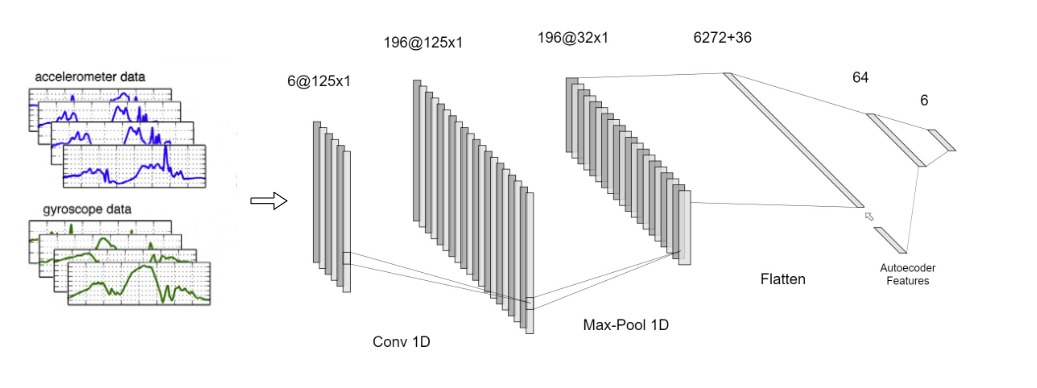
\includegraphics[width=1\textwidth]{images/full_architecture.jpg}
	\caption{Learning Framework}
	\label{fig:proposed-architecture}
\end{figure*}

In this section we will present our proposed architecture for HAR ``in
the wild'' problem. We will see how the autoencoder and the CNN are
trained, their parameters, and the optimization strategies adopted.

\subsection{Autoencoder}
\label{subsec:autoencoder}

In this section we describe the autoencoder model based on
\cite{vincent2010stacked}, \cite{gu2018locomotion} and
\cite{gao2019human}. An autoencoder is a type of artificial neural
network used to learn efficient data codings in an unsupervised
manner. The aim of an autoencoder is to learn a representation
(encoding) for a set of data by training the network to ignore signal
noise. Given $X = [ \boldsymbol{a}_v, \boldsymbol{a}_o,
  \boldsymbol{a}_l, \boldsymbol{g}_v, \boldsymbol{g}_o,
  \boldsymbol{g}_l ]^T$ as a $6\text{x}125$ matrix and $\x$ as the
column vector $750\text{x}1$ obtained by reshaping $\boldsymbol{X}$ we
can define the autoencoder in two blocks. The first block is the
encoder which is a function of the input:
\begin{equation}
  f_\theta(\x) = s(\boldsymbol{W}\x + \boldsymbol{b})
\end{equation}
where $\theta = \{ \boldsymbol{W}, \boldsymbol{b} \}$ with
$\boldsymbol{W}$ the weight matrix and $\boldsymbol{b}$ the bias
vector, while $s$ is the sigmoid activation function. We
can derive $\y = f_\theta(\x)$ as the output of this
layer. The second block is the decoder where the input is
reconstructed back starting from the code obtained by the encoder
\begin{equation}
  g_{\theta'}(\y) = s(\boldsymbol{W'}\y + \boldsymbol{b'})
\end{equation}
where $\theta' = \{ \boldsymbol{W'}, \boldsymbol{b'} \}$ are the
parameters obtained from previous step. Thus, the reconstructed input
is $\z = g_{\theta'}(\y)$. What we want to minimize is the distance
between $\x$ and $\z$ w.r.t. a distance measure with a loss function
like MSE.

The main goal of the autoencoder for this application is to extract
useful representations of input signal in few features and this is
done by looking at the autoencoder's code, i.e., the output of the
encoder block:
\begin{equation}
  \Phi_{\text{e}} = \y.
\end{equation}

The autoencoder follows the strucutre reported in
Fig. \ref{fig:encoder-structure} and is based on a Neural Network
architecture. The encoder is built with an input layer of
$6\text{x}125$ neurons reshaped as a vector $750\text{x}1$, one hidden
layer with 150 neurons and ReLU activation function, and an output
layer, i.e, the code, of $36\text{x}1$ neurons with sigmoid activation
function. The decoder replicates the same strucutre of the encoder but
reversed, where the activaction function on the output layers is the
identity.
\begin{figure}[h]
  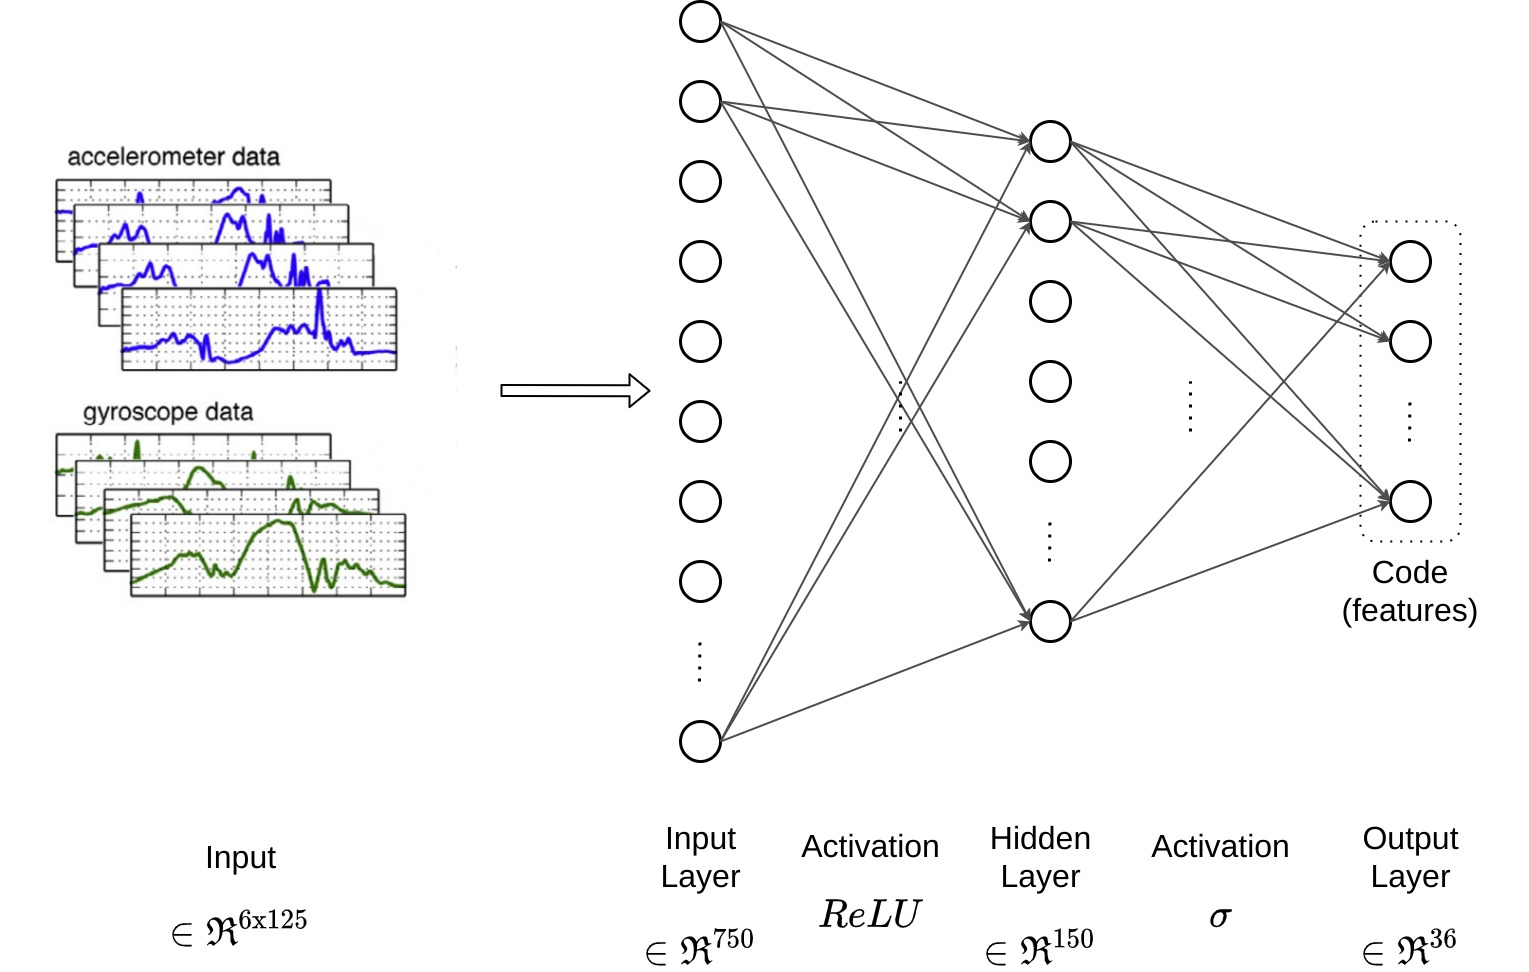
\includegraphics[width=0.5\textwidth]{images/encoder.jpg}
  \caption{(Auto)-encoder structure}
  \label{fig:encoder-structure}
\end{figure}

In order to search for best autoencoder model we tune hyperarameters
with grid search technique. Results are reported in
Tab. \ref{tab:ae-hyperparams} where values that performs well on the
validation dataset are reported in bold.
\begin{table}
  \centering
  \begin{tabular}{lp{4cm}}
    \hline
    Hyperparameter & Values \\
    \hline
    code size & \{2, 3, 4, 5, 6, 12, 18, 24, 30, \textbf{36}, 42, 48, 54, 60, 72\} \\
    batch size & \{32, \textbf{128}\} \\
    epochs & \{\textbf{150}, 200\} \\
    \hline
  \end{tabular}
  \caption{Grid-search for best hyperparameters on autoencoder}
  \label{tab:ae-hyperparams}
\end{table}
The best model used to be the one with a relatively small code
size: from 24 to 36 features which is also a good thing as we do not
want the autoencoder to learn the identity, but only to keep useful
information.

Even if the primary goal for this autoencoder is to automatically
extract features from signal for the main CNN model, we implement also
two simple classifiers in order to directly use autoencoder's feature
and check their effectiveness. We adopt two different classifier.  The
first is a K-Nearest Neighbors (KNN)\footnote{FIXME: citare quel paper
  di rossi dove parlava della clusterizzazione sulle feat. autoencoder
  che non trovo piu} clustering algorithm, and we perform clustering
on encoder's code. The idea here is that autoencoder should extract
relevant features which may be similar class by class. We perform a
grid search for metric and number of neighbors, values are reported in
Tab.~\ref{tab:knn-grid-search}. We select the euclidean distance
measure and $5$ as number of neighbors.
\begin{table}
  \centering
  \begin{tabular}{p{2cm}p{4.5cm}}
    \hline
    Hyperparameters & Values \\
    \hline
    Distance measure & \{\textbf{euclidean}, manhattan, chebyshev, minkowski, standardize euclidean, mahalanobis\} \\
    Number of neighbors & \{3, 4, \textbf{5}, 6, 7, 8\} \\
    \hline
  \end{tabular}
  \caption{Grid-search for KNN classifier}
  \label{tab:knn-grid-search}
\end{table}
The second classifier instead is based on a Feed Forward Neural
Network with two dense layers of $100$ neurons with $0.1$ dropout on
each and ReLU activaction function, while the last is a dense layer of
$5$ neurons with softmax activaction function. The network is trained
with Adam optimizer and categorical crossentropy loss function. We do
not further investigate this model as this is out of our scope.

\subsection{Convolutional neural network}
\label{subsec:cnn}

Parlare dell'archittettura proposta suddividendola in layer e alla fine dell'ottimizzazione adottata.

The final CNN architecture proposed in this work is shown in Fig. \ref{fig:proposed-architecture}. We decided to start with the architecture proposed in work \cite{chen2020deep} and we tried to improve it, augmenting the CNN with the encoder extracted features. CNN architecture are very powerfull when dealing with images, but they were proven to be a good features extractors also for motion data. A CNN is composed of essentially two parts: the first-one is in charge of extract features performing a dimensionality reduction over the input data, though a series of convolution and max pooling layers, and the second part of the CNN is responsible to give the final classification with usually a single fully-connected layer. Original data, collected from smartphone sensors are pre-processed according to what previously described in Sec. \ref{sec:processing_architecture}. Our input matrix presented to our CNN is the matrix \mbox{$ \boldsymbol{X} = [ \boldsymbol{a_{v}}^{c}, \boldsymbol{a_{h}}^{c}, \boldsymbol{a_{l}}^{c}, \boldsymbol{g_{v}}^{c}, \boldsymbol{g_{h}}^{c}, \boldsymbol{g_{l}}^{c}]$} wich is formed by acclerometer and gyroscopes signals, linearly interpolated at 50 samples/second  per channel with a fixed time-window of $2.5s$ with orientation independent transformation and data centering. Note that this matrix has a dimension $n \times 6$, due to the fact that TensorFlow Convolutional Layers work with input dimension of $(batch\_size, samples, channel)$.

In detail we have the following stacked layers:
\begin{itemize}
	\item \textbf{CL1}: The first convolutional is performing a Convolution 1D over the input signal. It composed of 196 filters of size ($1\times16$). Since, a convolution is defined over all the input channels, in this layer we are capturing relation among accellerometer and gyroscope data. The stride is set to 1, and the padding is configured as 'same' to have the same output dimension as te original one. After the convolution operation, we apply a $ReLU(x)=\max(0,x)$ activation function to learn non-linear correlation between signals and extract richer features. Furthermore, even if we are dealing with a small architecture, $ReLU$ activation function could prevent vanishing gradient problems, is less prone to overfitting since it induces the sparsity in the hidden units and it is extremely fast to compute, making it perfect when dealing with low computational resources.
	\item \textbf{MP1}: After the a convolutional layer, usually it is apply a max-pooling or average-pooling layer to reduce and summarize the obtained representation. We decided to use max-pool layer of size ($1\times4$), reducing by 4 times the original input shape. We call this new features representation with $ \Phi_{\text{c}} $
	\item \textbf{FC1}: After the convolutional layer and the max-pooling layer, the output of these layer is flattened into 6272 neurons. At this stage we decided to concatenate the encoder extracted features $ \boldsymbol{\Phi_{\text{e}}} $ with the Convolutional ones named $\boldsymbol{\Phi_{\text{c}}}$, creating our complete features vector $\boldsymbol{\Phi} = (\boldsymbol{\Phi_{\text{c}}}, \boldsymbol{\Phi_{\text{e}}})^T$ that is presented to the final fully-connected layer to perform the classification.
	\item \textbf{FC2-3}: These two finals layers are composed of 64 dense neuron and 6 dense neurons, respectively. These two final layers are used to perform the classification of the activity. For the FC2 we use the $ReLU$ activation function and for the final classification we apply the \textit{soft-max} activation function, which computes probability distribution over the predicted classes.
\end{itemize}

As for optimization techniques we decided to use dropout and $l_2$-regularization. The later techniques are commonly used in these types of architectures, yield a much more performance in the test set and so in generalation capabilities, preventing overfitting. We apply a dropout rate of 0.05 to the last fully-connected layer and we also apply a the $l_2$-regularization to all the fully connected layers. We have try with different hyper-parameters values for these two applied techniques, without any substantial changes in classification performance on the test set. Finally the parameters of the network are optimized using Adam CITE, a modification of stochastic gradient descent that also incorporates Momentum.
